% !TeX root = ../../../main.tex
\begin{figure}[!t]
\ChTwoFloatContents
    {ch02:fig:toyDataset}% label for whole figure
    {\caption{Synthetic dataset: panel (a) shows the only 4 possible time series trajectories (each true embedding vector state has a unique color-shape combination; there are 10 such states); every time series has 3 time steps and belongs to one of two classes \textcolor{red}{red}/\textcolor{blue}{blue}. Panels (b)-(e) show learned embedding spaces of four methods; only \ChTwoSmallCaps{Temporal-SCL} correctly recovers the 10 ground truth states. A version of this figure with embeddings of all methods evaluated is in Fig.~\ref{ch02:fig:toyDataset_result_complete}.
    }}% caption for whole figure
    {%
     
        \subfigure[Ground truth]{%
            \label{ch02:fig:toyDataset_Raw}
            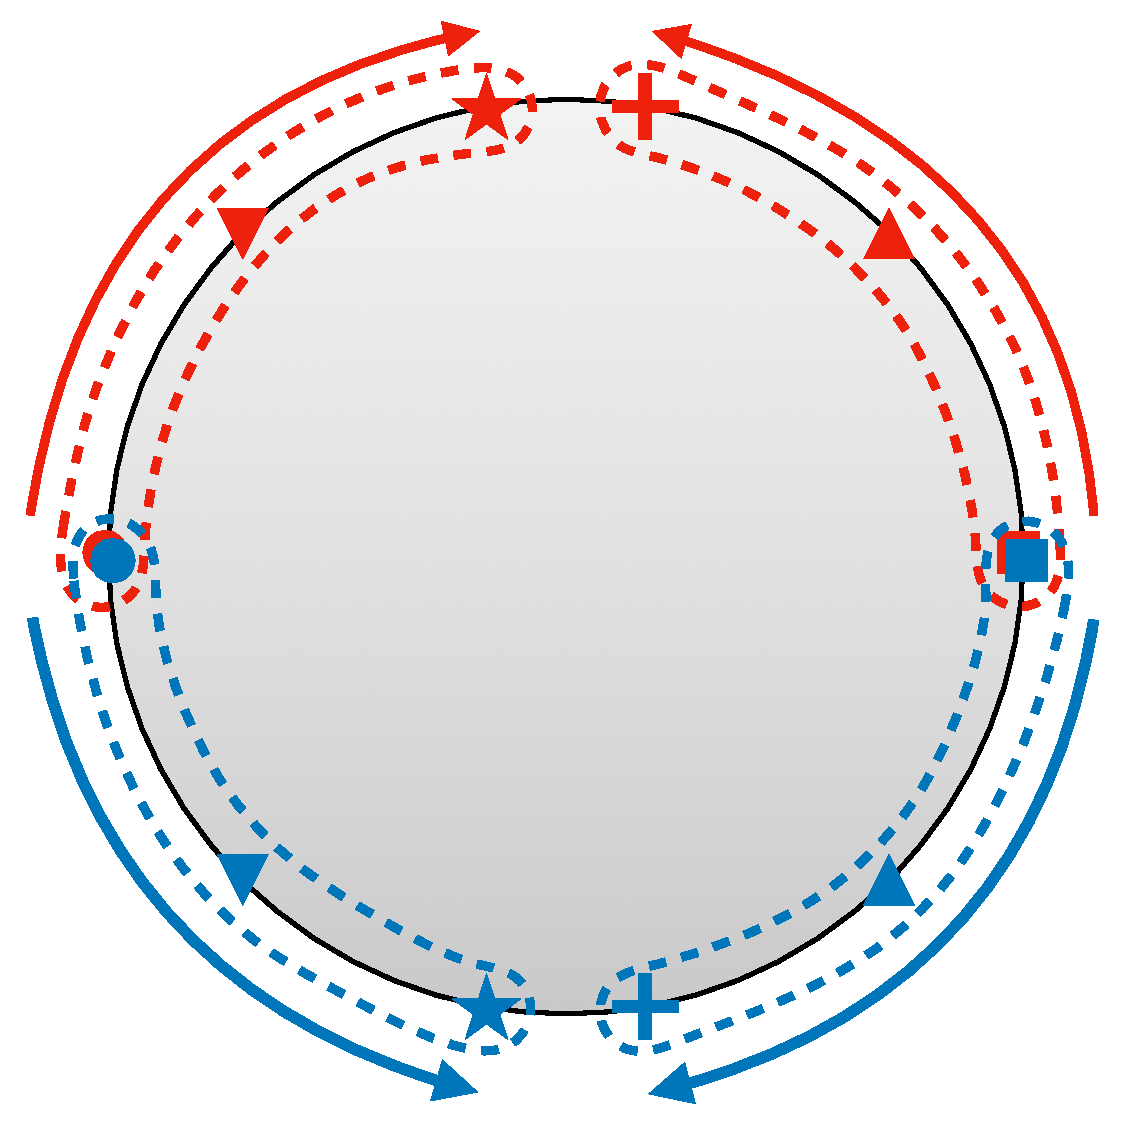
\includegraphics[width=0.195\linewidth]{Chapters/chapter-02/images/synthetic.pdf}
        }
        % \subfigure[RETAIN]{%
        %     \includegraphics[width=0.18\linewidth]{Figures/Embedding_RETAIN.png}
        % }
        \subfigure[Transformer]{%
            \label{ch02:fig:synth-transformer}% label for this sub-figure
            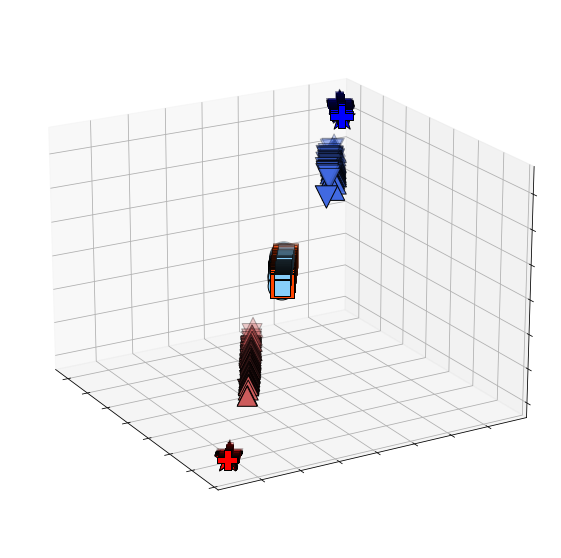
\includegraphics[width=0.18\linewidth]{Chapters/chapter-02/images/Embedding_Transformer.png}
        }
        \subfigure[T-Phenotype]{%
            \label{ch02:fig:synth-tphenotype}% label for this sub-figure
            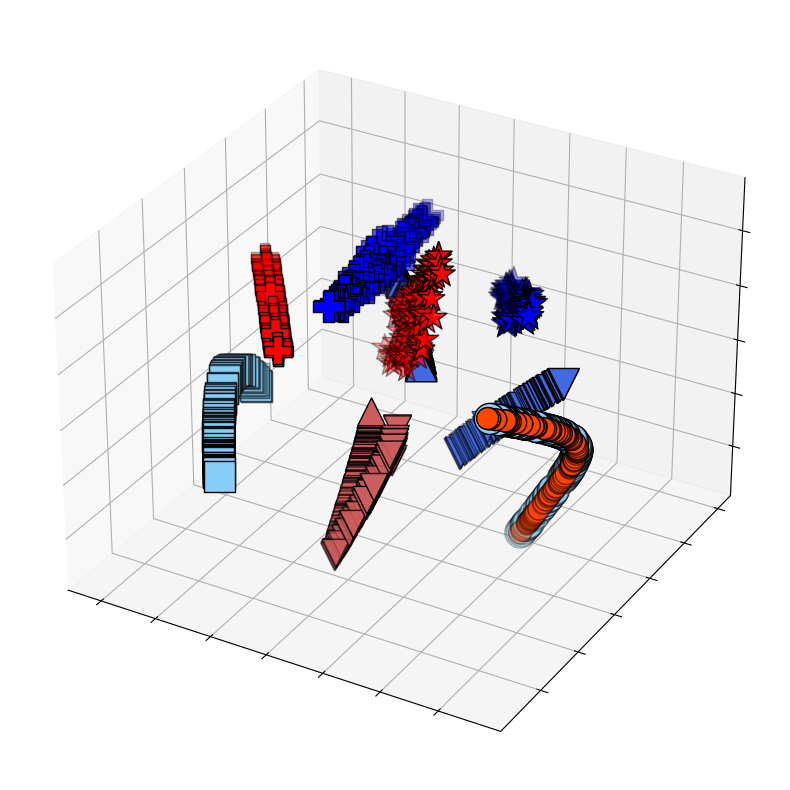
\includegraphics[width=0.18\linewidth]{Chapters/chapter-02/images/Embedding_TPhenotype.png}
        }
        \subfigure[\small\ChTwoSmallCaps{Temporal-SCL} \newline (no NN pairing)]{%
            \label{ch02:fig:synth-tscl-no-nnp}% label for this sub-figure
            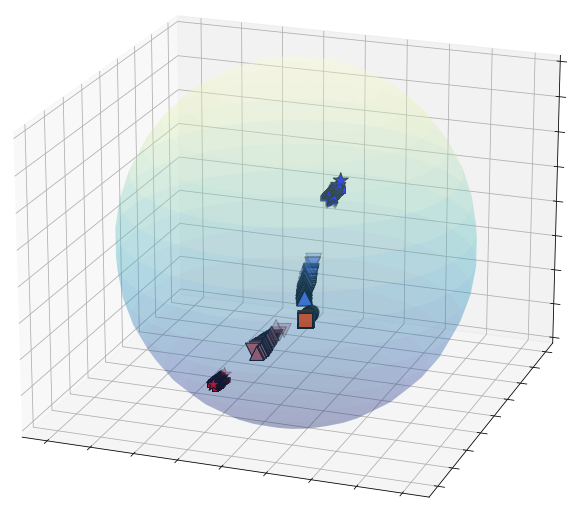
\includegraphics[width=0.18\linewidth]{Chapters/chapter-02/images/Embedding_NoKNN.png}
        }
        ~
        \subfigure[\small\ChTwoSmallCaps{Temporal-SCL}]{%
            \label{ch02:fig:synth-tscl}% label for this sub-figure
            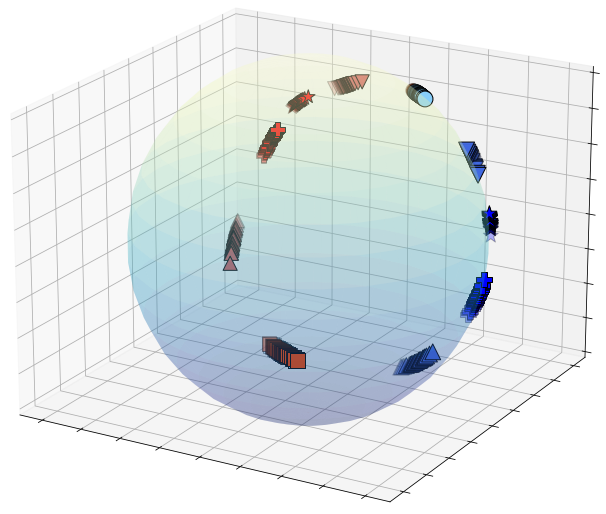
\includegraphics[width=0.18\linewidth]{Chapters/chapter-02/images/Embedding_TSCL.png}
        }
    }
\end{figure}